\documentclass[../../main.tex]{subfiles}
\begin{document}


{\bf [解]}
\paragraph{(1)}
下図のように各点をおく．ここで$|BC|=\ell,\angle ABC=\alpha, \angle ACB=\beta$である．

\begin{figure}[htb]
\centering
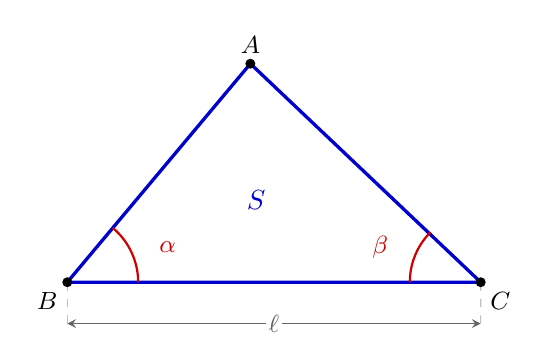
\begin{tikzpicture}[scale=1.5, >=stealth, every node/.style={font=\small}]

  % 頂点座標の設定 (例: BC = 3.5, 角 B = 50°, 角 C = 65°)
  \coordinate (B) at (0, 0);
  \coordinate (C) at (3.5, 0);
  % Aの座標計算
  \coordinate (A) at (1.55, 1.85);

  % 三角形の描画
  \draw[very thick, blue!80!black] (A) -- (B) -- (C) -- cycle;

  % 底辺 l の寸法表示
  \draw[<->, gray!80!black] (0, -0.35) -- (3.5, -0.35) node[midway, fill=white, inner sep=1pt] {$\ell$};
  \draw[dashed, gray!50] (B) -- (0, -0.4);
  \draw[dashed, gray!50] (C) -- (3.5, -0.4);

  % 角 B (\alpha) のアーク
  \draw[thick, red!80!black] (0.6, 0) arc[start angle=0, end angle=501/10, radius=0.6];
  \node[red!80!black] at (0.85, 0.3) {$\alpha$};

  % 角 C (\beta) のアーク
  \draw[thick, red!80!black] (2.9, 0) arc[start angle=180, end angle=135, radius=0.6];
  \node[red!80!black] at (2.65, 0.3) {$\beta$};

  % 頂点プロットとラベル
  \fill (A) circle (1.2pt) node[above] {$A$};
  \fill (B) circle (1.2pt) node[below left] {$B$};
  \fill (C) circle (1.2pt) node[below right] {$C$};

  % 面積 S のラベル
  \node[font=\bfseries, blue!80!black] at (1.6, 0.7) {$S$};

\end{tikzpicture}
\caption{底辺 $\ell$ と 2 角 $\alpha, \beta$ による三角形 $ABC$}
\end{figure}

正弦定理から
\begin{align}
\dfrac{AB}{\sin\beta}&=\dfrac{AC}{\sin\alpha}=\dfrac{\ell}{\pi-\sin(\alpha+\beta)}=\dfrac{\ell}{\sin(\alpha+\beta)} \quad\cdots\text{①}  \label{eq:1}
\end{align}
であるから，三角形ABCの面積$S$は
\begin{align}
S
 &=\dfrac{1}{2}AB\cdot AC\cdot\sin(\alpha+\beta) \\
 &=\dfrac{1}{2}\cdot\dfrac{\ell\sin\beta}{\sin(\alpha+\beta)}\cdot\dfrac{\ell\sin\alpha}{\sin(\alpha+\beta)}\cdot\sin(\alpha+\beta) \quad(\because\text{\cref{eq:1}}) \\
 &=\dfrac{\ell^2}{2}\cdot\dfrac{\sin\alpha\sin\beta}{\sin(\alpha+\beta)} \\
 &=\dfrac{\ell^2}{4}\cdot\dfrac{\cos(\alpha-\beta)-\cos(\alpha+\beta)}{\sin(\alpha+\beta)}
\end{align}
である．よって題意は示された．

\paragraph{(2)}
下図のように各点をおく．ここで$|AB|=2, |BC|=1, |CA|=\sqrt{3}$である．この時$\angle ACB=\angle R, \angle ABC=\dfrac{\pi}{3}$となる．
辺AB,BC,CA上（頂点は除く）にE,D,Fをとって三角形EDFが正三角形になるとする．この正三角形の一辺の長さを$x$, $\angle FDC=\theta$とおくと，
\begin{align}
 0 < \theta < \dfrac{\pi}{2} \label{eq:2}
\end{align}
である．

\begin{figure}[htb]
\centering
\begin{tikzpicture}[scale=2.2, >=stealth, every node/.style={font=\small}]

  % 頂点座標の設定
  % C = (0,0), B = (1,0), A = (0, sqrt(3))
  \coordinate (C) at (0, 0);
  \coordinate (B) at (1, 0);
  \coordinate (A) at (0, 1.732);

  % 正三角形 EDF の座標 (一辺 x, 角度 \theta)
  % D は BC 上, F は CA 上, E は AB 上
  % 例として \theta \approx 30° の配置
  \coordinate (D) at (0.6, 0);
  \coordinate (F) at (0, 0.346); % CD = x cos\theta, CF = x sin\theta
  \coordinate (E) at (0.43, 0.987);

  % 1. 直角三角形 ABC
  \draw[very thick, blue!80!black] (A) -- (B) -- (C) -- cycle;

  % 直角記号 (角 C)
  \draw[thick, gray!80!black] (0, 0.1) -- (0.1, 0.1) -- (0.1, 0);

  % 2. 内接する正三角形 EDF (塗りつぶし＋赤枠)
  \fill[pattern=north east lines, pattern color=black!40] (E) -- (D) -- (F) -- cycle;
  \draw[thick, red!80!black] (E) -- (D) -- (F) -- cycle;

  % 辺の長さ x のラベル (正三角形 EDF)
  \node[red!80!black, font=\scriptsize, right] at (0.32, 0.2) {$x$};

  % 3. 角のアークとラベル
  % 角 B = \pi/3 (60°)
  \draw[thick, gray!80!black] (0.8, 0) arc[start angle=180, end angle=120, radius=0.2];
  \node[font=\scriptsize] at (0.72, 0.1) {$\frac{\pi}{3}$};

  % 角 FDC = \theta
  \draw[thick, red!80!black] (0.45, 0) arc[start angle=180, end angle=150, radius=0.15];
  \node[red!80!black, font=\scriptsize] at (0.38, 0.07) {$\theta$};

  % 角 EDB = \pi - \pi/3 - \theta = 2\pi/3 - \theta
  % (図が煩雑にならないよう必要に応じて表示)

  % 4. 各辺の長さ表記 (AB=2, BC=1, CA=\sqrt{3})
  \node[left, font=\scriptsize] at (0, 0.866) {$\sqrt{3}$};
  \node[below, font=\scriptsize] at (0.5, 0) {$1$};
  \node[above right, font=\scriptsize] at (0.5, 0.866) {$2$};

  % 5. 頂点プロットとラベル
  \fill (A) circle (0.8pt) node[above left] {$A$};
  \fill (B) circle (0.8pt) node[below right] {$B$};
  \fill (C) circle (0.8pt) node[below left] {$C$};

  \fill[red!80!black] (D) circle (0.8pt) node[below] {$D$};
  \fill[red!80!black] (E) circle (0.8pt) node[above right] {$E$};
  \fill[red!80!black] (F) circle (0.8pt) node[left] {$F$};

\end{tikzpicture}
\caption{直角三角形 $ABC$ と内接する正三角形 $EDF$}
\end{figure}


$\triangle BDE$に正弦定理を用いて
\begin{align}
 &\dfrac{|BD|}{\sin\theta} = \dfrac{x}{\sin\dfrac{\pi}{3}} \\
\therefore 
 &|BD| = \dfrac{2}{3}\sqrt{3}\cdot x\sin\theta \label{eq:3}
\end{align}
である．また$\triangle CDF$に注目して
\begin{align}
 |CD| = |DF|\cos\theta = x\cos\theta \label{eq:4}
\end{align}
である．
$BD+CD=1$に\cref{eq:3,eq:4}を代入して
\begin{align}
\left(\dfrac{2}{3}\sqrt{3}\sin\theta+\cos\theta\right)x=1 \quad\cdots\text{①} \label{eq:5}
\end{align}
である．三角関数の合成より
\begin{align}
 \dfrac{2}{3}\sqrt{3}\sin\theta+\cos\theta = \sqrt{\dfrac{7}{3}}\sin(\theta+\theta_0)
\end{align}
である．ここで$\theta_0$は$\sin\alpha=\sqrt{3/7},\ \cos\alpha=2/\sqrt{7}$をみたす$0<\theta_0<\dfrac{\pi}{2}$の角である．
\cref{eq:2}と合わせて$\theta+\theta_0=\dfrac{\pi}{2}$となる$\theta$があるからこの時$x$は最小値
\begin{align}
 x = \dfrac{1}{\sqrt{\dfrac{7}{3}}\sin(\theta+\theta_0)} = \dfrac{1}{\sqrt{\dfrac{7}{3}}} = \sqrt{\dfrac{3}{7}}
\end{align}
をとる．この時三角形EDFの面積$T=\dfrac{\sqrt{3}x^2}{4}$は最小値
\begin{align}
 \min T=\dfrac{\sqrt{3}}{4}\cdot\dfrac{3}{7}=\dfrac{3\sqrt{3}}{28} 
\end{align}
をとる．

\end{document}
